\documentclass[12pt]{article}\usepackage{graphicx}
\graphicspath{{./figs/}}{}

\usepackage{amsmath,amssymb,amsfonts,amsthm}
\newcommand{\myvec}[1]{\ensuremath{\begin{pmatrix}#1\end{pmatrix}}}
%\providecommand{\norm}[1]{\lVert#1\rVert}3
\usepackage{listings}
\usepackage{watermark}
\usepackage{titlesec}
\usepackage{caption}
\let\vec\mathbf
\lstset{
frame=single, 
breaklines=true,
columns=fullflexible
}
\usepackage{atbegshi}% http://ctan.org/pkg/atbegshi
\AtBeginDocument{\AtBeginShipoutNext{\AtBeginShipoutDiscard}}
\let\vec\mathbf
\providecommand{\norm}[1]{\left\lVert#1\right\rVert}
\newcommand{\solution}{\noindent \textbf{Solution: }}
\newcommand{\mydet}[1]{\ensuremath{\begin{vmatrix}#1\end{vmatrix}}}
\title{\mytitle}
\begin{document}
\begin{center}
\title{\textbf{VECTOR ALGEBRA}}
\maketitle
\end{center}
\begin{enumerate}
\item\textbf{Problem statement :} Evaluate the product $\myvec{3\overrightarrow{a}-5\overrightarrow{b}}\cdot\myvec{2\overrightarrow{a}+7\overrightarrow{b}}$
\solution
\begin{align}
    \myvec{3\vec{a}-5\vec{b}}^{\top}\cdot\myvec{2\vec{a}+7\vec{b}}= 3\vec{a}^{\top}\cdot2\vec{a}+3\vec{a}^{\top}\cdot7\vec{b}-5\vec{b}^{\top}\cdot2\vec{a}-5\vec{b}^{\top}\cdot7\vec{b}
\end{align}
Properties of Vector
\begin{align}
    \vec{a}^{\top}\cdot\vec{a} = \norm{\vec{a}}^2
    \label{eq1}  
    \\
    \vec{a}^{\top}\cdot\vec{b} = \vec{b}^{\top}\cdot\vec{a}
    \label{eq2}
\end{align}
By using \eqref{eq1} and \eqref{eq2}
\begin{align}
    \myvec{3\vec{a}-5\vec{b}}^{\top}\cdot\myvec{2\vec{a}+7\vec{b}}^{\top} = 6\norm{\vec{a}}^2 +21\vec{a}^{\top}\cdot\vec{b}-10\vec{b}^{\top}\cdot\vec{a}-35\norm{\vec{b}}^2 \\
     =6\norm{\vec{a}}^2-35\norm{\vec{b}}^2+11\vec{a}^{\top}\cdot\vec{b}
\end{align}
\begin{figure}[!h]
 \begin{center}
  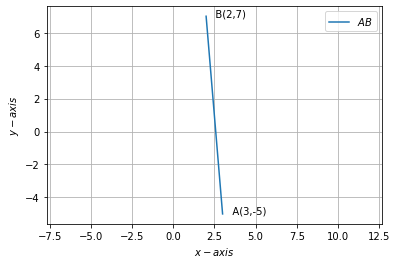
\includegraphics[width=\columnwidth]{./fig.png}
 \end{center}
\caption{}
\label{fig:Fig1}
\end{figure}
\end{enumerate}
\end{document}
